%
%===============>>  Ленотьева Модуль 7 <<=============
%
\setmodule{7}

%BEGIN_FOLD % ====>>_____ Занятие 1 _____<<====
\begin{class}[number=1]
	\begin{listofex}
		\item Занятие 1
	\end{listofex}
\end{class}
%END_FOLD

%BEGIN_FOLD % ====>>_____ Занятие 2 _____<<====
\begin{class}[number=2]
	\begin{listofex}
		\item На рисунке изображён график функции \( y=f(x) \) левая круглая скобка x правая круглая скобка . Какие из утверждений относительно этой функции неверны? Укажите их номера.
		\begin{figure}[h!]
			\centering
			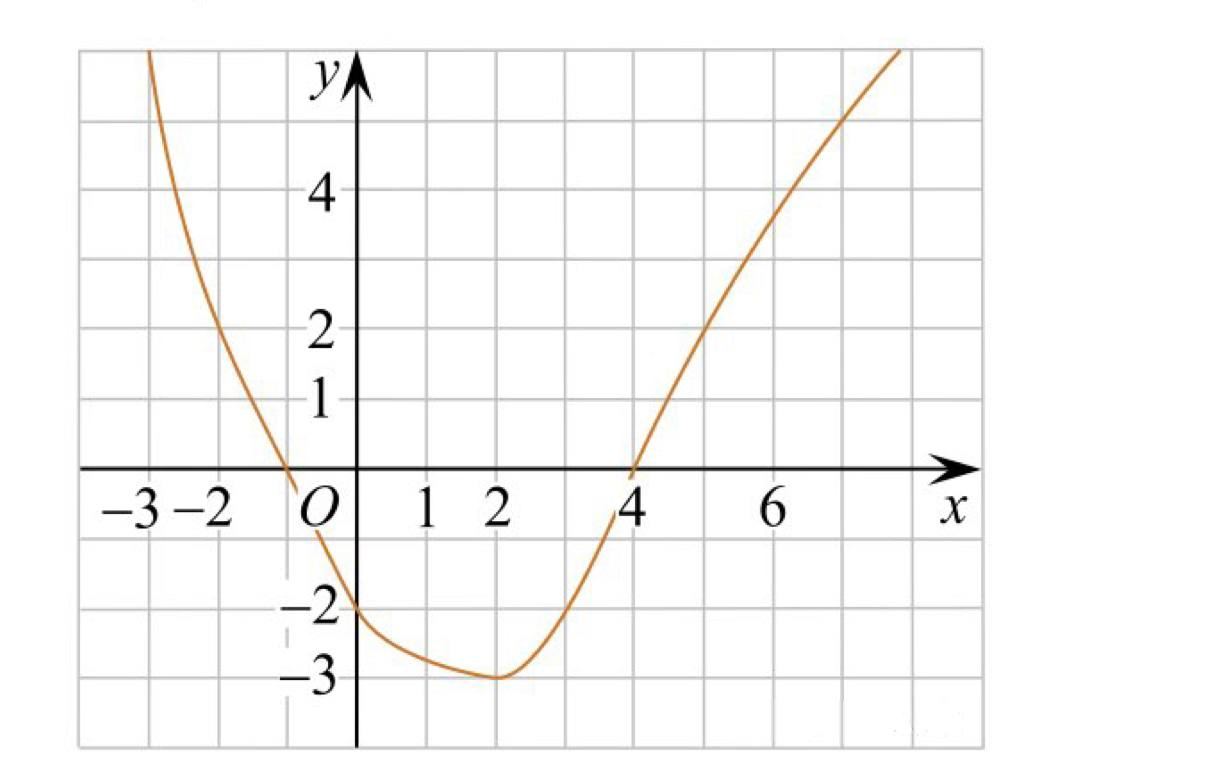
\includegraphics[width=0.4\linewidth]{../../../../../exercises/lists/pics/leontevaM7L2-1}
		\end{figure}
		\begin{tasks}(1)
			\task функция возрастает на промежутке  \( [-2; +\infty) \)
			\task \( f(3)> f(-3)  \)
			\task \( f(0) = -2 \)
			\task прямая y=2  пересекает график в точках \(  (-2; 2) \)  и \( (5; 2) \) 
		\end{tasks}
		\item На рисунке изображён график квадратичной функции \( y  =  f(x) \).
		\\
		Какие из следующих утверждений о данной функции неверны? Запишите их номера в порядке возрастания.
		\begin{figure}[h!]
			\centering
			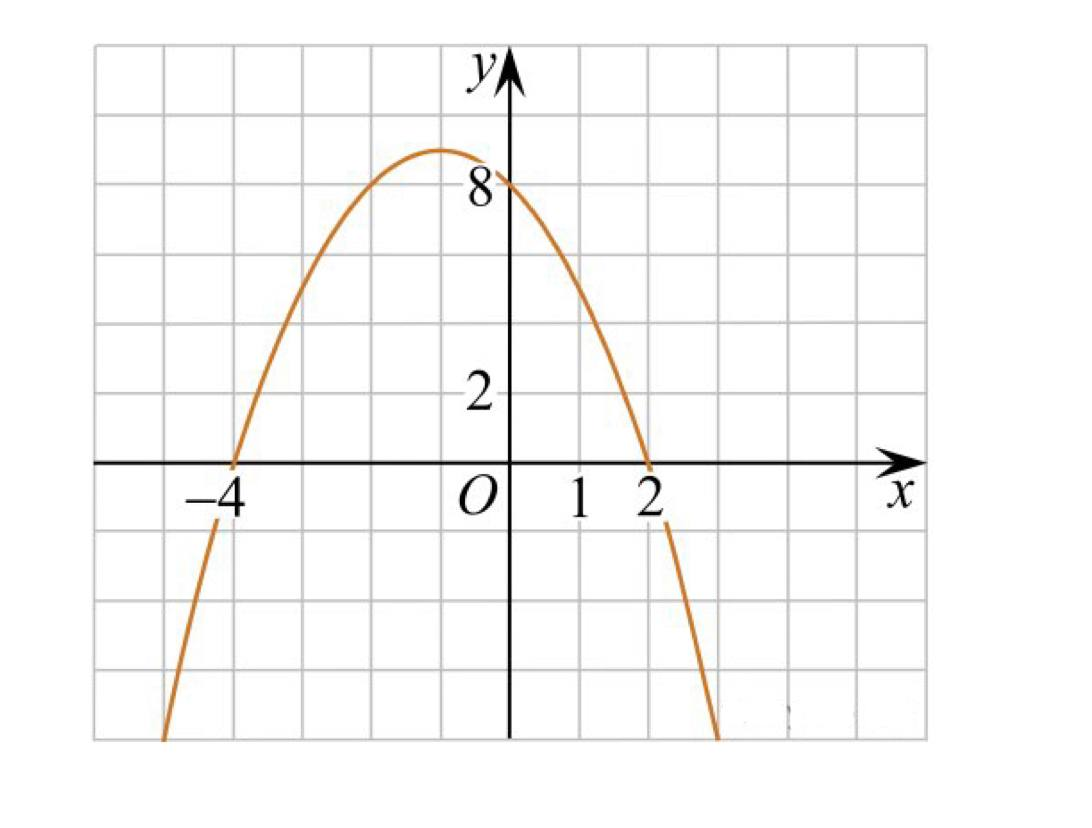
\includegraphics[width=0.4\linewidth]{../../../../../exercises/lists/pics/leontevaM7L2-2}
		\end{figure}
		\begin{tasks}(1)
			\task Функция возрастает на промежутке \( (-\infty;  -1 \)].
			\task Наибольшее значение функции равно \( 8 \).
			\task \( f(-4) \neq f(2) \).
		\end{tasks}
		\newpage
		\item На рисунке изображён график квадратичной функции \( y =  f(x) \).
		Какие из следующих утверждений о данной функции неверны? Запишите их номера.
		\begin{figure}[h!]
			\centering
			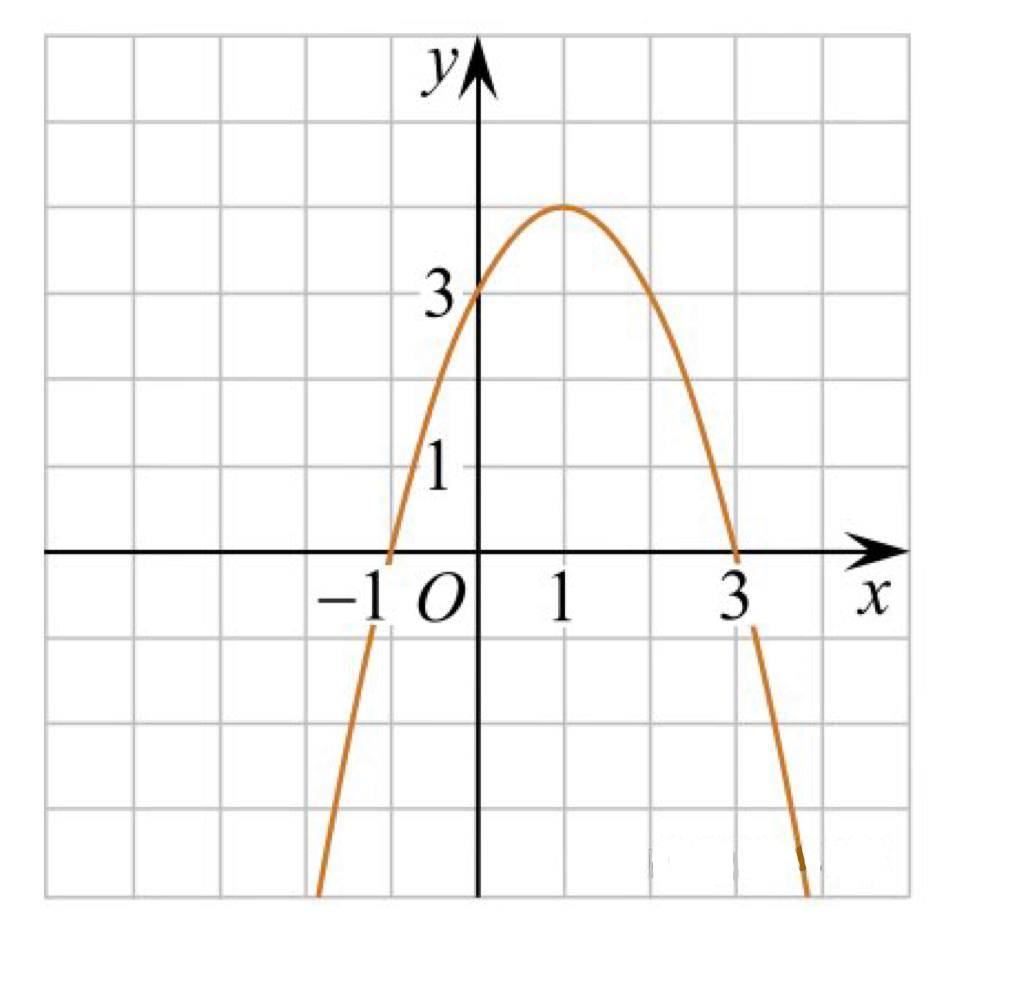
\includegraphics[width=0.4\linewidth]{../../../../../exercises/lists/pics/leontevaM7L2-3}
		\end{figure}
		\begin{tasks}(1)
			\task \( f(-1)=f(3) \).
			\task Наибольшее значение функции равно \( 3 \).
			\task \( f(x)>0  \) при  \( -1<x<3 \).
		\end{tasks}
		\item На рисунке изображён график квадратичной функции \( y = f(x) \).
		
		Какие из следующих утверждений о данной функции неверны? Запишите их номера.
		\begin{figure}[h!]
			\centering
			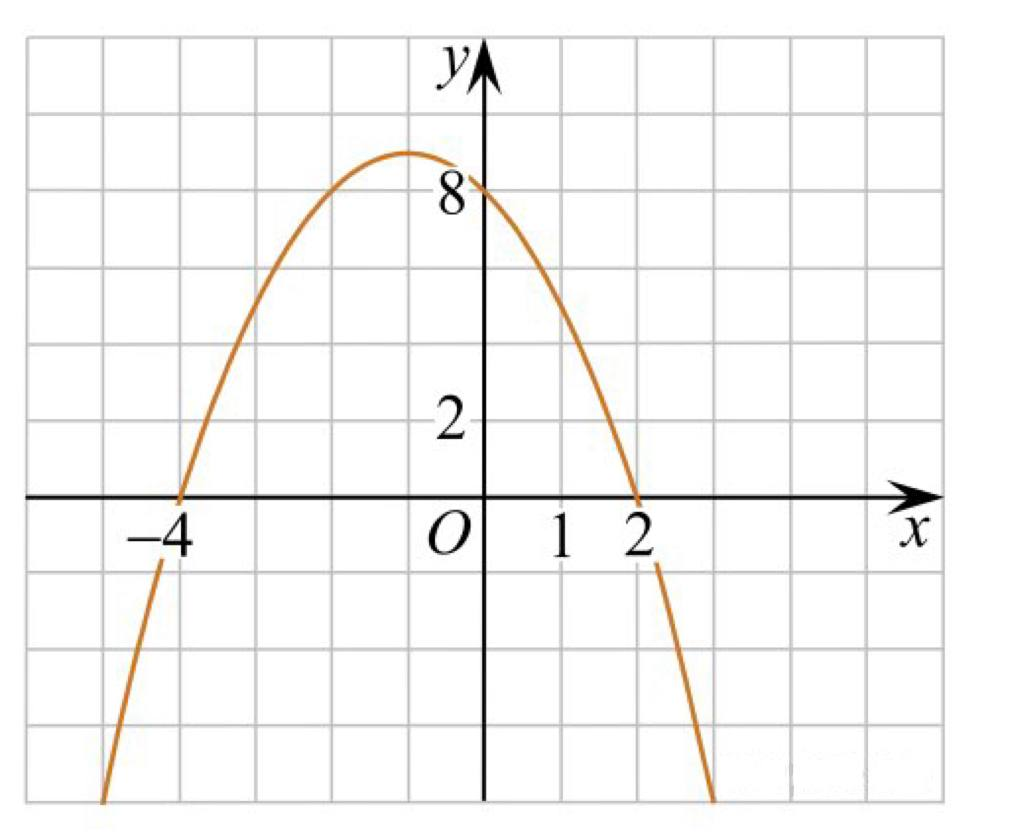
\includegraphics[width=0.4\linewidth]{../../../../../exercises/lists/pics/leontevaM7L2-4}
		\end{figure}
		\begin{tasks}(1)
			\task  Наибольшее значение функции равно \( 9 \).
			\task \( f(0)>f(1) \).
			\task \( f( x )>0 \) при \( x<0 \).
		\end{tasks}
		\newpage
		\item На рисунке изображён график функции \(  y = ax2 + bx + c \). Установите соответствие между утверждениями и промежутками, на которых эти утверждения выполняются. 
		\begin{figure}[h!]
			\centering
			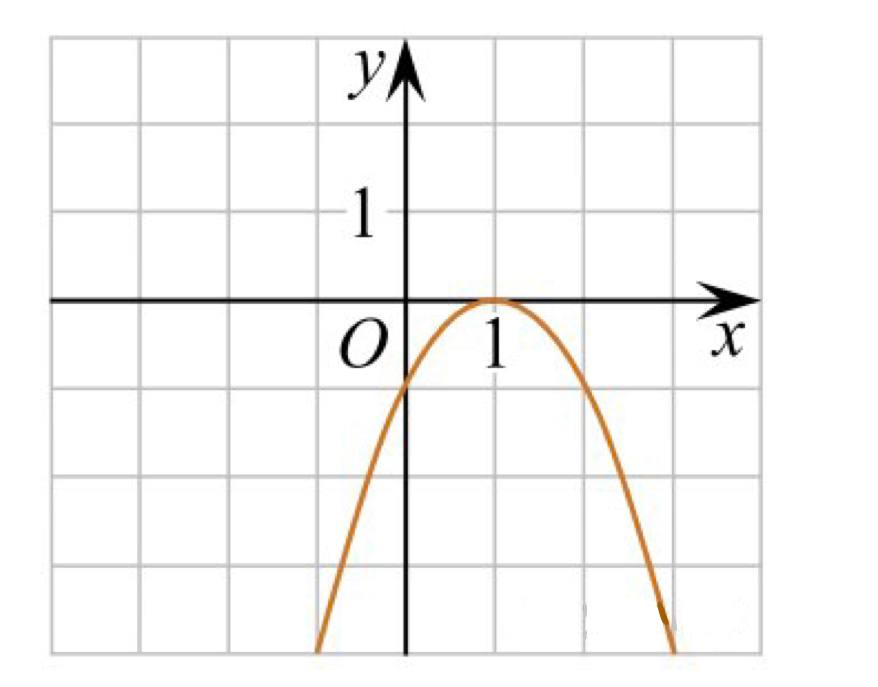
\includegraphics[width=0.3\linewidth]{../../../../../exercises/lists/pics/leontevaM7L2-5}
		\end{figure}
		\begin{tasks}(2)
			\task[] УТВЕРЖДЕНИЯ	 
			\task[]	ПРОМЕЖУТКИ
			\task[A)] функция возрастает на промежутке
			\task \( [1;2] \)
			\task[B)]функция убывает на промежутке
			\task \( [0;2] \)
			\task[]
			\task\( [-1;0] \)
			\task[]
			\task\( [-2;3] \)
		\end{tasks}
		\item 
		На рисунке изображён график функции \(  y = ax2 + bx + c \). Установите соответствие между утверждениями и промежутками, на которых эти утверждения выполняются. 
		\begin{figure}[h!]
			\centering
			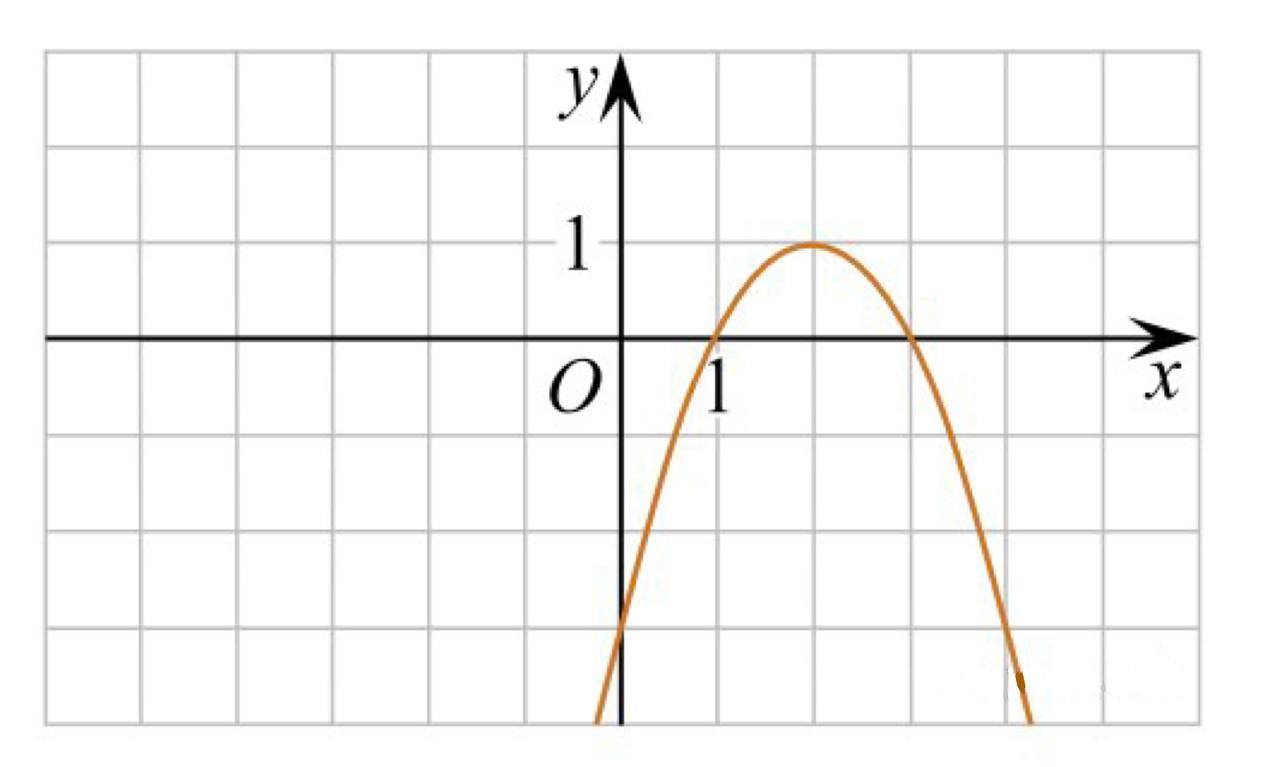
\includegraphics[width=0.3\linewidth]{../../../../../exercises/lists/pics/leontevaM7L2-6}
		\end{figure}
		\begin{tasks}(2)
			\task[] УТВЕРЖДЕНИЯ	 
			\task[]	ПРОМЕЖУТКИ
			\task[A)] функция возрастает на промежутке
			\task \( [0; 3] \)
			\task[B)]функция убывает на промежутке
			\task \( [-1; 1] \)
			\task[]
			\task\( [2; 4] \)
			\task[]
			\task\( [1; 4] \)
		\end{tasks}
		\item Найдите координаты вершины параболы \( y = 2x^{2} + 4x + 5 \).
		\item Найдите координаты вершины параболы\(  y = -x^{2} + 2x - 4 \).
		\item Найдите координаты вершины параболы\(  y = \dfrac{1}{3}x^{2}+x-1 \).
		\item Найти вершину параболы, заданной формулой \( y=2x^{2} - 8x + 5. \)
	\end{listofex}
\end{class}
%END_FOLD

%BEGIN_FOLD % ====>>_____ Занятие 3 _____<<====
\begin{class}[number=3]
	\begin{listofex}
		\item Один из смежных углов на \( 40^{\circ} \) больше другого. Найдите эти углы.
		\item Внутри развернутого угла \( PNE \) провели луч  \( NR \). Найди каждый из двух  образовавшихся углов, если один из них в \( 4 \) раза больше другого.  
		\item При пересечении двух прямых образовались такие углы, что сумма двух из них равна \( 100^{\circ} \). Найди все углы.
		\item В треугольнике \( ABC \)    \( AB=BC \),   внешний угол при вершине \( B  \)  равен \( 138^{\circ} \).   Найдите \( \angle C \).   Ответ дайте в градусах.
		\item В треугольнике \( ABC \)   \( \angle B= 39^{\circ} \) ,  \(  AB  =BC \).   Найдите внешний угол при вершине \( A \).   Ответ дайте в градусах.
		\item В равнобедренном треугольнике \( ABC \)  внешний угол при вершине \( B \) равен \( 86^{\circ} \). Найдите наименьший из внутренних углов этого треугольника. Ответ дайте в градусах.
		\item В треугольнике \( ABC \)  \( \angle A = 52^{\circ} \), \( \angle C = 71^{\circ} \).На продолжении стороны \( BC \)   за точку \( B \)   отложен отрезок \( BD = AB \).   Найдите \( \angle D \)   треугольника \( ABD \).   Ответ дайте в градусах.
		\item В треугольнике \( ABC \)   \( \angle A = 22^{\circ} \),   внешний угол при вершине \( C \)   равен \( 130^{\circ} \).   Найдите \( \angle B \).   Ответ дайте в градусах.
		\item Найдите углы треугольника, зная, что внешние углы при двух его вершинах равны \( 130^{\circ} \) и \( 140^{\circ} \).
		\item Один из углов, образовавшихся при пересечении двух прямых, равен \( 45^{\circ} \). Найди остальные углы.
		\item Биссектрисы углов \( N \) и \( M \) треугольника \(  MNP \) пересекаются в точке \( A \). Найдите \( \angle NAM \), если \( \angle N=84^{\circ} \), а \( \angle M=42\degree \). 
		\item Углы треугольника относятся как \(  2:8:35 \). Найдите меньший из них. Ответ дайте в градусах.
		\item Два угла треугольника равны \( 58^{\circ} \) и \( 72^{\circ} \). Найдите тупой угол, который образуют высоты треугольника, выходящие из вершин этих углов. Ответ дайте в градусах.
		\item В треугольнике \( ABC \) \( CH \)  — высота, \( AD \)  — биссектриса, \( O \) — точка пересечения прямых \( CH \) и \( AD \),  \( \angle BAD \) равен \( 26^{\circ} \). Найдите \( \angle AOC \). Ответ дайте в градусах.
	\end{listofex}
\end{class}
%END_FOLD

%BEGIN_FOLD % ====>>_____ Занятие 4 _____<<====
\begin{class}[number=4]
	\begin{listofex}
		\item Один из острых углов прямоугольного треугольника на \( 24^{\circ} \) больше другого. Найдите углы данного треугольника. Ответ дайте в градусах.
		\item В треугольнике \( ABC \): \( C=90^{\circ} \), \( AB=8 \) и \( BC=5 \). Найдите \( AC \).
		\item Дан прямоугольный треугольник \( ABC \), \( \angle C=90^{\circ} \), и \( AC=3 \), \( BC=4 \). Найдите длину \( AB \).
		\item Два острых угла прямоугольного треугольника относятся как \( 4:5 \). Найдите больший острый угол. Ответ дайте в градусах.
		\item В прямоугольном треугольнике катет и гипотенуза равны \( 40 \) и \( 41 \) соответственно. Найдите другой катет этого треугольника.
		\item Катеты прямоугольного треугольника равны \( 8 \) и \( 15 \). Найдите гипотенузу этого треугольника.
		\item Катеты прямоугольного треугольника равны \( 18 \) и \( 24 \). Найдите высоту, проведенную к гипотенузе.
		\item В треугольнике \( ABC \) угол \( C \) равен \( 90^{\circ} \), \( M \)  — середина стороны \( AB \), \( AB  =  20 \), \( BC = 10 \). Найдите \( CM \).
		\item Биссектриса равностороннего треугольника равна  \( 4\sqrt{3} \). Найдите сторону этого треугольника.
		\item Диагонали ромба равны \( 14 \) см и \( 48 \) см. Найдите сторону ромба.
		\item В треугольнике два угла равны \( 45\degree \) и \( 90\degree \), а большая сторона — \( 20 \) см. Найдите две другие стороны треугольника и запишите их сумму .
		\item Стороны прямоугольника равны \( 8 \) см и \( 12 \) см. Найдите его диагональ.
	\end{listofex}
\end{class}
%END_FOLD

%BEGIN_FOLD % ====>>_ Домашняя работа 2 _<<====
\begin{homework}[number=2]
	\begin{listofex}
		\item Биссектрисы углов \( N \) и \( M \) треугольника \( MNP\) пересекаются в точке \( A \). Найдите \( \angle NAM \), если \( \angle N=84^{\circ }  \), а \( \angle M= 42^{\circ} \).
		\item
		\begin{minipage}[t]{\bodywidth}
			Углы, отмеченные на рисунке одной дугой, равны. Найдите угол \( \alpha \). Ответ дайте в градусах.
		\end{minipage}
		\hspace{0.02\linewidth}
		\begin{minipage}[t]{\picwidth}
			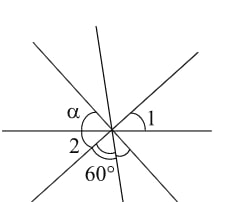
\includegraphics[align=t, width=0.8\linewidth]{../../../../../exercises/lists/pics/leontevaM7H2-1}
		\end{minipage}
	\item
	\begin{minipage}[t]{\bodywidth}
		 Углы, отмеченные на рисунке одной дугой, равны. Найдите угол \( \alpha \). Ответ дайте в градусах.
	\end{minipage}
	\hspace{0.02\linewidth}
	\begin{minipage}[t]{\picwidth}
		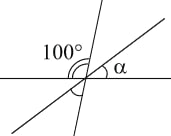
\includegraphics[align=t, width=0.8\linewidth]{../../../../../exercises/lists/pics/leontevaM7H2-2}
	\end{minipage}
	\item 
	\begin{minipage}[t]{\bodywidth}
		На плоскости даны четыре прямые. Известно, что \( \angle 1 = 120^{\circ} \), \( \angle 2 = 60^{\circ} \), \( \angle 3 = 55^{\circ} \). Найдите \( \angle 4 \). Ответ дайте в градусах.
	\end{minipage}
	\hspace{0.02\linewidth}
	\begin{minipage}[t]{\picwidth}
		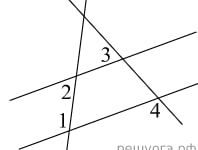
\includegraphics[align=t, width=0.8\linewidth]{../../../../../exercises/lists/pics/leontevaM7H2-3}
	\end{minipage}
	\item На рисунке изображён график квадратичной функции \( y  =  f(x) \).
	Какие из следующих утверждений о данной функции неверны? Запишите их номера
	\begin{figure}[h!]
		\centering
		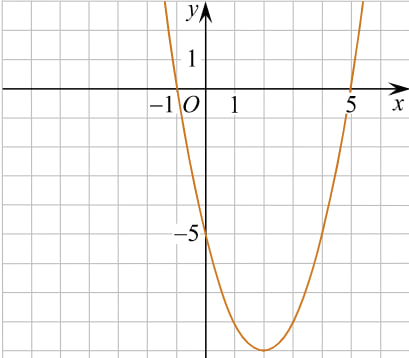
\includegraphics[width=0.4\linewidth]{../../../../../exercises/lists/pics/leontevaM7H2-4}
	\end{figure}
	\begin{tasks}(1)
		\task  1)  \( f(x)<0 \) при \( -1<x<5 \).
		\task Функция возрастает на промежутке \( [2; +\infty) \).
		\task Наименьшее значение функции равно \( -5 \).
	\end{tasks}
	\end{listofex}
\end{homework}
%END_FOLD

%BEGIN_FOLD % ====>>_____ Занятие 5 _____<<====
\begin{class}[number=5]
	\begin{listofex}
		\item В равнобедренном треугольнике \( ABC \) с основанием \( AC \) внешний угол при вершине C равен \( 74\degree \). Найдите величину угла \( ABC \). Ответ дайте в градусах.
		\item В треугольнике \( ABC \) проведена биссектриса \( AL \), угол \( ALC \) равен \( 112\degree \), угол \( ABC \) равен \( 106\degree \). Найдите угол \( ACB \). Ответ дайте в градусах.
		\item 
		\begin{minipage}[t]{\bodywidth}
			На рисунке изображен прямоугольный треугольник. Найдите его площадь.
		\end{minipage}
		\hspace{0.02\linewidth}
		\begin{minipage}[t]{\picwidth}
			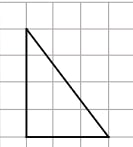
\includegraphics[align=t, width=0.8\linewidth]{../../../../../exercises/lists/pics/leontevaM7L5-1}
		\end{minipage}
		\item Площадь треугольника \( S \) (м\( ^{2} \))  можно вычислить по формуле \( S= \dfrac{1}{2}ah \),  где \( a \)  — сторона треугольника, \( h  \) — высота, проведенная к этой стороне (в метрах). Пользуясь этой формулой, найдите сторону \( a \), если площадь треугольника равна \( 28 \) м\( ^{2} \), а высота \( h \) равна \( 14  \)м.
		\item Периметр равнобедренного треугольника равен \( 16 \), а боковая сторона  — \( 5 \). Найдите площадь треугольника.
		\item В треугольнике одна из сторон равна \( 10 \), а опущенная на нее высота  — \( 5 \). Найдите площадь треугольника.
		\item В равнобедренном треугольнике \( ABC AC=BC \). Найдите \( AC \), если высота \( CH=12 \), \( AB=10 \).
		\item Высота равностороннего треугольника равна \( 15 \sqrt{3} \). Найдите его периметр.
		\item Катеты прямоугольного треугольника равны \( 35 \) и \( 120 \). Найдите высоту, проведенную к гипотенузе.
		\item У треугольника со сторонами \( 16 \) и \( 2 \) проведены высоты к этим сторонам. Высота, проведённая к первой стороне, равна \( 1 \). Чему равна высота, проведённая ко второй стороне?
		\item В треугольнике \( ABC \) проведены медиана \( BM \) и высота \( BH \) . Известно, что \( AC  =  84 \) и \( BC  =  BM \). Найдите \( AH \).
		\item Медиана равностороннего треугольника равна \( 11 \) корень из \( 3 \). Найдите сторону этого треугольника.
	\end{listofex}
\end{class}
%END_FOLD

%BEGIN_FOLD % ====>>_____ Занятие 6 _____<<====
\begin{class}[number=6]
	\begin{listofex}
		\item \begin{tasks}(2)
			\task 
				\( \begin{cases}
					3x-1<x+5
					\\
					7x+4>3x
				\end{cases} \)
			\task \( \begin{cases}
				4(9x+3)-9(4x+3)>3x
				\\
				(x-2)(x+9)<0
			\end{cases} \)
		\end{tasks}
		\end{listofex}
		\begin{definit}
		\textbf{Синусом} острого угла прямоугольного треугольника называется отношение противолежащего катета к гипотенузе.
		\end{definit}
		\begin{definit}
		\textbf{Косинусом} острого угла прямоугольного треугольника называется отношение прилежащего катета к гипотенузе.
		\end{definit}
		\begin{listofex}[resume]
		\item В треугольнике \( ABC \) угол \( C \) равен \( 90 \) градусов, \( AC=6 \), \( AB=20 \). Найдите \( \sin B \).
		\item  В треугольнике \( ABC \) угол \( C \) равен \( 90 \) градусов, \( BC=9 \), \( AB=20 \). Найдите \( \cos B \).
		\item Найдите синус, косинус углов \( A \) и \( B \) треугольника \( ABC \) с прямым углом \( C \), если:
		\begin{tasks}(2)
			\task \( BC=8 \), \( AB=17 \)
			\task \( BC=21 \), \( AC=20 \)
			\task \( BC=1 \), \( AC=2 \)
		\end{tasks}
		\item В треугольнике \( ABC \) угол \( C \) прямой, \( BC=8 \), \( \sin A=0,4 \). Найдите \( AB \).
		\item В треугольнике \( ABC \) угол \( C \) прямой, \( AC=15 \), \( \cos A=\dfrac{5}{7} \). Найдите \( AB \).
		\item В треугольнике \( ABC \) угол \( C \) равен \( 90\degree \), \( BC=12 \), \( \sin A=\dfrac{4}{11} \). Найдите \( AB \).
		\item Катеты прямоугольного треугольника равны \( \sqrt{15} \) и \( 1 \). Найдите синус наименьшего угла этого треугольника.
		\item В треугольнике \( ABC \) угол \( C \) равен \( 90\degree \), \( \sin A=\dfrac{4}{5} \), \( BC=9 \). Найдите \( AB \).
		\item  Есть прямоугольный треугольник \( ABC \), где \( \angle C=90^{\circ} \), и \( AC=7 \), \( AB=25 \). Найдите длину \( BC \).
	\end{listofex}
\end{class}
%END_FOLD

%BEGIN_FOLD % ====>>_ Домашняя работа 3 _<<====
\begin{homework}[number=3]
	\begin{listofex}
		\item В треугольнике \( ABC \) угол \( C \) прямой, \( BC=12 \), \( \sin A=\dfrac{6}{13} \). Найдите \( AB \).
		\item В треугольнике \( ABC \) угол \( C \) прямой, \( BC=15 \), \( \cos B=\dfrac{18}{30} \). Найдите \( AB \).
		\item  Высота треугольника равна \( 10 \) и образует с прилежащими сторонами углы \( 45\degree \) и \( 60\degree \). Найдите стороны треугольника.
		\item Основание равнобедренного треугольника равно \( 16 \), боковая сторона равна \( 10 \). Чему равна высота проведенная к основанию этого треугольника?
		\item Боковая сторона равнобедренного треугольника равна \( 13 \), а длина основания равна \( 10 \). Найдите площадь этого треугольника.
	\end{listofex}
\end{homework}
%END_FOLD

%BEGIN_FOLD % ====>>_____ Занятие 7 _____<<====
\begin{class}[number=7]
	\begin{listofex}
		\item Найдите значение выражения \( 4^{-10}\cdot(4^{3})^{4} \).
		\item Найдите значение выражения \( (\sqrt{31 }-3)(\sqrt{31}+3) \).
		\item Упростите выражение \( (a-3)^{2}-a(5a-6) \) и найдите его значение при \( a=-\dfrac{1}{2} \).  В ответе запишите найденное значение.
	\end{listofex}
	\begin{definit}
		\textbf{Тангенсом} острого угла прямоугольного треугольника называется отношение противолежащего катета к прилежащему катету.
	\end{definit}
	\begin{definit}
		\textbf{Котангенсом} острого угла прямоугольного треугольника называется отношение прилежащего катета к противолежащему катету.
	\end{definit}
	\begin{definit}
		\textbf{Основное тригонометрическое тождество:} \[\sin^2\alpha+\cos^2\alpha=1\]
	\end{definit}
	\begin{listofex}[resume]
		\item
		\begin{minipage}[t]{\bodywidth}
			Вычислите значения синуса, косинуса, тангенса и котангенса отмеченных углов.
		\end{minipage}
		\hspace{0.02\linewidth}
		\begin{minipage}[t]{\picwidth}
			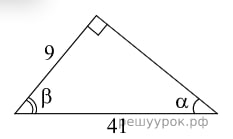
\includegraphics[align=t, width=0.8\linewidth]{../../../../../exercises/lists/pics/leontevaM7L7-1}
		\end{minipage}
	\end{listofex}
		\begin{definit}
			\begin{tasks}(3)
				\task[] \[\dfrac{\sin\alpha}{\cos \alpha}=\tg \alpha\] 
				\task[] \[\dfrac{\cos\alpha}{\sin \alpha}=\ctg \alpha\] 
				\task[] \[\ctg\alpha\cdot\tg \alpha = 1\]
			\end{tasks}
		\end{definit}
	\begin{listofex}[resume]
		\item Найдите синус, косинус и тангенс и котангенс углов \( A \) и \( B \) треугольника \( ABC \) с прямым углом \( C \), если:
		\begin{tasks}(2)
			\task \( BC=5 \), \( AB=13 \)
			\task \( BC=28 \), \( AC=21 \)
			\task \( BC=8 \), \( AC=6 \)
		\end{tasks}
		\item В треугольнике \( ABC \) \( \angle C = 90\degree  \) \( \cos A = \dfrac{5}{12} \). Найдите \( \sin A \), \( \tg A \), \( \ctg A \).
		\item В треугольнике \( ABC \) \( AC = BC = 8,2 \), \(  \tg A=\dfrac{9}{40} \). Найдите высоту \( CH \).
		\item В треугольнике одна из сторон равна \( 10 \), другая равна \( 10\sqrt{3} \), а угол между ними равен \( 60\degree \). Найдите площадь треугольника.
		\item В треугольнике одна из сторон равна \( 12 \), другая равна \( 10 \), а тангенс угла между ними равен  \( \dfrac{\sqrt{2}}{4}\). Найдите площадь треугольника.
		\item В треугольнике \( ABC \) угол \( C \) равен \( 90\degree \), \( \sin A=\dfrac{4}{5} \), \( AC=9 \). Найдите \( AB \).
		\item В прямоугольном треугольнике \( ABC \) \( \angle C=90\degree \) \( \cos B=\dfrac{2}{7} \), \( AC=21 \). Найдите \( AB \).
		\item В прямоугольном треугольнике \( MNK \) \( \angle N = 90\degree \), \( \sin M = 0,6 \), \( MN=9 \). Найдите длину \( NK \).
	\end{listofex}
\end{class}
%END_FOLD

%BEGIN_FOLD % ====>>_ Занятие 8 _<<====
\begin{class}[number=8]
	\begin{listofex}
		\item Найдите значение выражения   \( \dfrac{27b^{2}+108b+108}{b}:\left( \dfrac{6}{b}+3 \right) \) при \( b = - \dfrac{4}{9}\). 
		\item Найдите значение выражения \( (a^{3}-25a )\left( \dfrac{1}{a+5}-\dfrac{1}{a-5} \right)\) при \( a =-39 \).
		\item В ромбе \( ABCD \) угол \( D \) равен \( 140\degree \). Определите чему равены углы треугольника \( АОD \) (\( О \) – точка пересечения диагоналей).
		\item Периметр ромба равен \( 40 \), а один из углов равен \( 30\degree \). Найдите площадь ромба.
		\item Сторона ромба равна \( 34 \), а острый угол равен \( 60\degree \). Высота ромба, опущенная из вершины тупого угла, делит сторону на два отрезка. Каковы длины этих отрезков?
		\item Периметр ромба равен \( 24 \), а косинус одного из углов равен  \( \dfrac{2 \sqrt{2}}{3} \).  Найдите площадь ромба.
		\item \begin{minipage}[t]{\bodywidth}
			Найдите площадь параллелограмма, изображённого на рисунке.
		\end{minipage}
		\hspace{0.02\linewidth}
		\begin{minipage}[t]{\picwidth}
			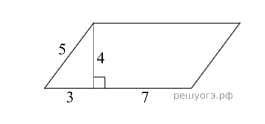
\includegraphics[align=t, width=0.8\linewidth]{../../../../../exercises/lists/pics/leontevaM7L8-1}
		\end{minipage}
		
		
		
		\item Периметр параллелограмма равен \( 16 \) см. Чему равны стороны параллелограмма, если известно, что одна его сторона в \( 3 \) раза больше другой?
		\item Биссектриса угла \( D \) параллелограмма \( ABCD \) пересекает сторону \( BC \) в точке \( M \), \( BM:MC = 4:3 \). Найдите периметр параллелограмма, если \( BC = 28 \) см
		\item Диагональ \( BD \) параллелограмма \( ABCD \) образует с его сторонами углы, равные \( 65\degree \) и \( 50\degree \). Найдите меньший угол параллелограмма.
		\item Разность углов, прилежащих к одной стороне параллелограмма, равна \( 40\degree \). Найдите меньший угол параллелограмма. Ответ дайте в градусах.
		\item Площадь параллелограмма равна \( 40 \), а две его стороны равны \( 5 \) и \( 10 \). Найдите его высоты. В ответе укажите большую высоту.
		\item Найдите величину острого угла параллелограмма \( ABCD \), если биссектриса угла \( A \) образует со стороной \( BC \) угол, равный \( 15\degree \). Ответ дайте в градусах.
	\end{listofex}
\end{class}
%END_FOLD